%%%%%%%%%%%%%%%%%%%%%%%%%%%%%%%%%%%%%%%%%
% Jacobs Landscape Poster
% LaTeX Template
% Version 1.0 (29/03/13)
%
% Created by:
% Computational Physics and Biophysics Group, Jacobs University
% https://teamwork.jacobs-university.de:8443/confluence/display/CoPandBiG/LaTeX+Poster
% 
% Further modified by:
% Nathaniel Johnston (nathaniel@njohnston.ca)
%
% This template has been downloaded from:
% http://www.LaTeXTemplates.com
%
% License:
% CC BY-NC-SA 3.0 (http://creativecommons.org/licenses/by-nc-sa/3.0/)
%
%%%%%%%%%%%%%%%%%%%%%%%%%%%%%%%%%%%%%%%%%

%----------------------------------------------------------------------------------------
%	PACKAGES AND OTHER DOCUMENT CONFIGURATIONS
%----------------------------------------------------------------------------------------

\documentclass[final]{beamer}

\usepackage[scale=1.24]{beamerposter} % Use the beamerposter package for laying out the poster
\usepackage{gb4e}
\usepackage{color}
\usepackage[labelformat=empty]{caption}
\usepackage[normalem]{ulem}
\usepackage{amsfonts}
\usepackage{graphicx}
\usepackage{tikz}
\usepackage[square, numbers]{natbib}
%\usepackage{algpseudocode}
\usepackage{algorithm}

\usetikzlibrary{calc}
\usetikzlibrary{shapes}
\usetikzlibrary{arrows}
\usetikzlibrary{fit,positioning}

\usetheme{confposter} % Use the confposter theme supplied with this template

\setbeamercolor{block title}{fg=BreakfastGreen,bg=white} % Colors of the block titles
\setbeamercolor{block body}{fg=black,bg=white} % Colors of the body of blocks
\setbeamercolor{block alerted title}{fg=white,bg=BreakfastBlue!90} % Colors of the highlighted block titles

\setbeamercolor{block alerted body}{fg=black,bg=BreakfastBlue!10} % Colors of the body of highlighted blocks
% Many more colors are available for use in beamerthemeconfposter.sty

%-----------------------------------------------------------
% Define the column widths and overall poster size
% To set effective sepwid, onecolwid and twocolwid values, first choose how many columns you want and how much separation you want between columns
% In this template, the separation width chosen is 0.024 of the paper width and a 4-column layout
% onecolwid should therefore be (1-(# of columns+1)*sepwid)/# of columns e.g. (1-(4+1)*0.024)/4 = 0.22
% Set twocolwid to be (2*onecolwid)+sepwid = 0.464
% Set threecolwid to be (3*onecolwid)+2*sepwid = 0.708

\newlength{\sepwid}
\newlength{\onecolwid}
\newlength{\twocolwid}
\newlength{\threecolwid}
\setlength{\paperwidth}{48in} % A0 width: 46.8in
\setlength{\paperheight}{36in} % A0 height: 33.1in
\setlength{\sepwid}{0.024\paperwidth} % Separation width (white space) between columns
\setlength{\onecolwid}{0.22\paperwidth} % Width of one column
\setlength{\twocolwid}{0.464\paperwidth} % Width of two columns
\setlength{\threecolwid}{0.708\paperwidth} % Width of three columns
\setlength{\topmargin}{-0.5in} % Reduce the top margin size
%-----------------------------------------------------------

\usepackage{graphicx}  % Required for including images

\usepackage{booktabs} % Top and bottom rules for tables

%----------------------------------------------------------------------------------------
%	TITLE SECTION 
%----------------------------------------------------------------------------------------

\title{MAD Style: Multivalent Authorship Detection (MAD) Topic Models} % Poster title

\author{David Dohan, Charles Marsh, Shubhro Saha, Max Simchowitz} % Author(s)

\institute{Princeton University, Department of Computer Science} % Institution(s)

%----------------------------------------------------------------------------------------

\begin{document}

\addtobeamertemplate{block end}{}{\vspace*{2ex}} % White space under blocks
\addtobeamertemplate{block alerted end}{}{\vspace*{2ex}} % White space under highlighted (alert) blocks

\setlength{\belowcaptionskip}{2ex} % White space under figures
\setlength\belowdisplayshortskip{2ex} % White space under equations

\begin{frame}[t]  % The whole poster is enclosed in one beamer frame

\begin{columns}[t] % The whole poster consists of three major columns, the second of which is split into two columns twice - the [t] option aligns each column's content to the top

\begin{column}{\sepwid}\end{column} % Empty spacer column

\begin{column}{\onecolwid} % The first column

%----------------------------------------------------------------------------------------
%	OBJECTIVES
%----------------------------------------------------------------------------------------

\begin{alertblock}{Goals}
\begin{itemize}
\item Classify author writing style in a wide range of media.
\item Extract compact representation of stylistic tendency.
\item Determine which features are most indicative of writing style.
\end{itemize}
\end{alertblock}

%----------------------------------------------------------------------------------------
%	INTRODUCTION
%----------------------------------------------------------------------------------------

\begin{block}{Introduction}

In the \textit{authorship detection} problem, one is given:
\begin{itemize}
\item A set of documents labeled (by author) on which to train.
\item A set of anonymized documents to classify.
\end{itemize} Methods for authorship detection traditionally depended on careful feature extraction and rather black-box methods. Hence, they rely on extensive domain specific knowledge, and can be difficult to decipher. Here, we present the \textit{MAD Topic Model}, which uses  syntactic and stylometric n-gram features (e.g., part-of-speech tags, meter). MAD fits separate topic models to each of these ngram vocabularies, and then combines the models with a multiclass logistic regression classifier. After fitting the topic model parameters, new data can be classified using the multiclass component. 

INSERT GRAPHIC

\end{block}



%----------------------------------------------------------------------------------------

\end{column} % End of the first column

\begin{column}{\sepwid}\end{column} % Empty spacer column

\begin{column}{\twocolwid} % Begin a column which is two columns wide (column 2)

\begin{columns}[t,totalwidth=\twocolwid] % Split up the two columns wide column

\begin{column}{\onecolwid}\vspace{-.6in} % The first column within column 2 (column 2.1)

%----------------------------------------------------------------------------------------
%	MATERIALS
%----------------------------------------------------------------------------------------

\begin{block}{Data}

To collect data for training and testing, we wrote Python scrapers for Project Gutenberg, Nassau Weekly, and Quora. We selected these three data sources for their diversity in topic, language, and length. Our Project Gutenberg dataset features fictional story excerpts from five, public-domain authors. The Nassau Weekly dataset features over 550 articles from about 200 authors. On the higher end, the Quora dataset features over 1600 comments from roughly 100 popular Quora users. The challenge posed for our authorship models is to detect consistent features in such a variety of contexts.

\end{block}

%----------------------------------------------------------------------------------------

\end{column} % End of column 2.1

\begin{column}{\onecolwid}\vspace{-.6in} % The second column within column 2 (column 2.2)

%----------------------------------------------------------------------------------------
%	METHODS
%----------------------------------------------------------------------------------------

\begin{block}{Features}

\begin{center}
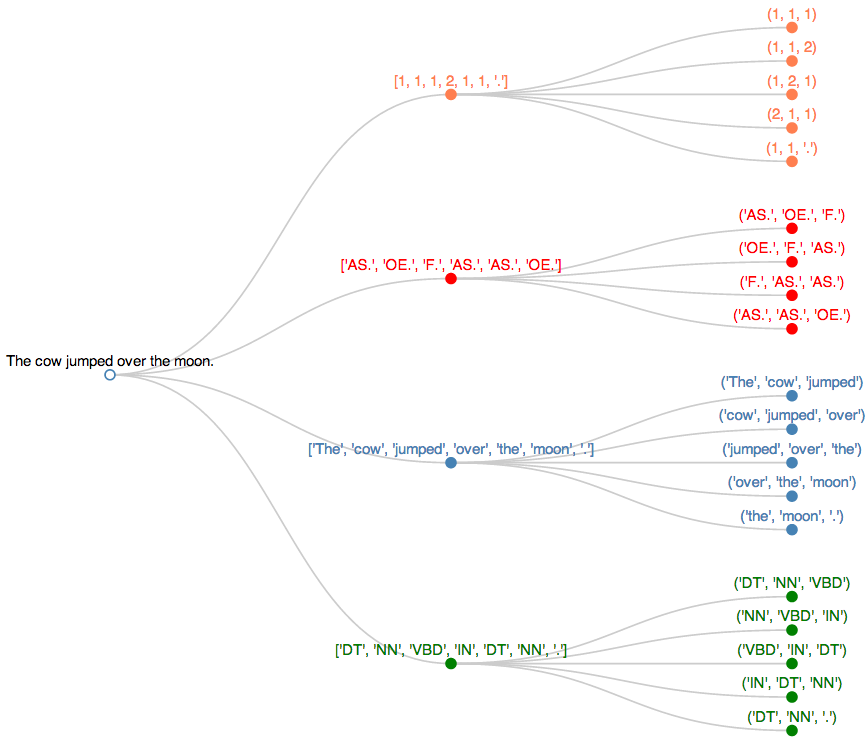
\includegraphics[width=\linewidth]{dendrogram.png}
\end{center}

\end{block}

%----------------------------------------------------------------------------------------

\end{column} % End of column 2.2

\end{columns} % End of the split of column 2 - any content after this will now take up 2 columns width

%----------------------------------------------------------------------------------------
%	IMPORTANT RESULT
%----------------------------------------------------------------------------------------

\begin{alertblock}{Summary}

The Multivalence Authorship Detection (MAD) Topic Model extends Latent Dirichlet Allocation \citep{Blei2003} to identify authorship in documents with many separate types (``multivalent") of count features. MAD is ``doubly supervised''--it includes a multi-class logistic regression as in \cite{Blei2007}--and also fits per-author Dirichlet distributions for each feature type. We test the MAD Topic Model on several real world corpora using a variety of $n$-gram features, including part-of-speech, syllable stress, and sequences of word lengths.
\end{alertblock} 

%----------------------------------------------------------------------------------------

\begin{columns}[t,totalwidth=\twocolwid] % Split up the two columns wide column again

\begin{column}{\onecolwid} % The first column within column 2 (column 2.1)

%----------------------------------------------------------------------------------------
%	MATHEMATICAL SECTION
%----------------------------------------------------------------------------------------

\begin{block}{Model}
\begin{figure}[h!]
  \centering
  \begin{tikzpicture}
  \tikzstyle{main}=[circle, minimum size = 10mm, thick, draw =black!80, node distance = 16mm]
  \tikzstyle{connect}=[-latex, thick]
  \tikzstyle{box}=[rectangle, draw=black!100]
    \node[main, fill = white!100] (theta)  {$\theta$ };
    \node[main] (alpha) [left=of theta] { $\alpha$};
    \node[main] (z) [right=of theta] {$z$};
    \node[main, fill = black!10] (w) [right=of z] {$w$};
    \node[main] (beta) [above=of z]{$\beta$};
    \node[main] (lambda) [left=of beta]{$\lambda$};
    \node[main] (y) [right=of w, fill = white!100, xshift = -6mm]{$y$};
    \node[main] (eta) [above=of y, xshift = 28mm,yshift=-2mm]{$\eta$};
    \path (alpha) edge [connect] (theta)
          (theta) edge [connect] (z)
          (z) edge [connect] (w)
          (lambda) edge [connect] (beta)
          (beta) edge [connect] (w)
          (eta) edge [connect] (y)
          (w) edge [connect] (y);
    \node[rectangle, inner sep=8mm, fit= (z) (w),label=below right:N, yshift = 10mm, xshift=3mm] {};
	\node[rectangle, inner sep=8mm,draw=black!100, fit= (z) (w), yshift = -6mm] {};
	 \node[rectangle, inner sep=8mm, fit= (beta),label=above right:k, yshift = -14mm, xshift=-15mm] {};
	\node[rectangle, inner sep=8mm,draw=black!100, fit= (beta), yshift = 2mm] {};
	\node[rectangle, inner sep=16mm, fit= (theta) (z) (w) (y),label=below:M, yshift = 4mm, xshift=-50.5mm] {};
	\node[rectangle, inner sep=16mm, draw=black!100, fit = (theta) (z) (y) (w), yshift = -12mm, xshift=16] {};
	\node[rectangle, inner sep=20mm, fit= (alpha) (theta) (z) (w) (y),label=below left:A, yshift = 8mm, xshift=-40mm] {};
	\node[rectangle, inner sep=20mm, draw=black!100, fit = (alpha) (theta) (z) (w) (y), yshift = -13mm, xshift=16] {};
	\node[rectangle, inner sep=28mm, fit = (lambda) (beta) (alpha) (theta) (z) (w), label=above right:T, yshift = -30mm, xshift=65] {};

	\node[rectangle, inner sep=28mm, draw=black!100, fit = (lambda) (beta) (alpha) (theta) (z) (w), yshift = -13mm, xshift=16] {};

    %\node[rectangle, inner sep=4.4mm, draw=black!100, fit= (x) (iota)  (beta) (r) ,label=below right:N,yshift=-3mm ] {};
    %\node[rectangle, inner sep=3.0mm, draw=black!100, fit= (x) ,label=below left:K] {};
  \end{tikzpicture}
  \caption{Graphical Model for the MAD Topic Model}
\end{figure}
\small The MAD topic model combines the SLDA algorithm presented in \cite{wang2009simultaneous} with the Author Topic Model in \cite{rosen2004author}, and extending both to account for multiple word types. The model is variational inference, following coordinate ascent updates in \cite{wang2009simultaneous}. Stochastic variational inference was also tested, but proved impractical for these rather small data sets. 

\end{block}

%----------------------------------------------------------------------------------------

\end{column} % End of column 2.1

\begin{column}{\onecolwid} % The second column within column 2 (column 2.2)

%----------------------------------------------------------------------------------------
%	RESULTS
%----------------------------------------------------------------------------------------

\begin{block}{Results}


\small
\indent Unfortunately, preliminary results show that which MAD fares far worse as using the same features with another classification scheme. This is consistent with \cite{...}, which suggests that a Pitman-Yor process better captures power law frequencies in language use than Dirichlet methods. Nevertheless, MAD's topic models over the $n$-gram stylistic features can be used to extract compact representations of stylistic tendency and discern which features are most indicative of individual writing style.

\end{block}

%----------------------------------------------------------------------------------------

\end{column} % End of column 2.2

\end{columns} % End of the split of column 2

\end{column} % End of the second column

\begin{column}{\sepwid}\end{column} % Empty spacer column

\begin{column}{\onecolwid} % The third column

%----------------------------------------------------------------------------------------
%	CONCLUSION
%----------------------------------------------------------------------------------------

\begin{block}{Visualization}

Replace this with some visualization.

\end{block}

%----------------------------------------------------------------------------------------
%	ADDITIONAL INFORMATION
%----------------------------------------------------------------------------------------

\begin{block}{Conclusion}

Our (short) conclusion.

\end{block}

%----------------------------------------------------------------------------------------
%	ACKNOWLEDGEMENTS
%----------------------------------------------------------------------------------------

\setbeamercolor{block title}{fg=BreakfastRed,bg=white} % Change the block title color

\begin{block}{References}
\small
\bibliography{poster}
\bibliographystyle{plainnat}

\end{block}

\begin{center}

\includegraphics[width=0.5\linewidth]{PU-long.jpg}
\end{center}

%----------------------------------------------------------------------------------------

\end{column} % End of the third column

\end{columns} % End of all the columns in the poster

\end{frame} % End of the enclosing frame

\end{document}
